\documentclass[a4paper,12pt]{article}


\usepackage{natbib}

\usepackage{float}

\usepackage[utf8]{inputenc}
\usepackage[bottom]{footmisc}

%Rajoute des régles de typo
\usepackage[french]{babel}
%Change l'accent
\usepackage[T1]{fontenc}
\usepackage{hyperref}
\usepackage{enumitem}
\usepackage{amsmath,amssymb}

\usepackage{color}

\usepackage{graphicx,xcolor}
\usepackage{subcaption}
\usepackage{geometry}
\geometry{left=1.5cm, right=1.5cm, bottom=2cm, }
\newcommand{\rmq}[1]{\textcolor{red}{#1}}

%Pour les définitions
\usepackage{amsthm}
\newtheorem{mydef}{Definition}

\begin{document}

	\newcommand{\HRule}{\rule{\linewidth}{0.5mm}}

	\begin{titlepage}

		\center

		\textsc{\LARGE Sorbonne université}\\[1.5cm] % Name of your university/college

        \begin{minipage}{0.4\textwidth}
		\begin{flushleft} \large
		\end{flushleft}
		\end{minipage}




		\textsc{\huge \bfseries Rapport de ARF}\\[.5cm]

		\HRule \\[0.4cm]
		{ \huge \bfseries TME 1 - 6 }\\[0.4cm]
		\HRule \\[4cm]

		{ \huge \textsc{Samu Tamminen} }

		\vfill
		Année 2017-2018
	\end{titlepage}



\newpage
\tableofcontents
\newpage

\section{TME 1 : Arbres de décision, sélection de modèles}

\subsection{Q1.3 Interpretation de l'entropie}
Calculer également la différence entre l’entropie et l’entropie conditionnelle pour chaque attribut.
A quoi correspond une valeur de 0 ? une valeur de 1 ? Quel est le meilleur attribut pour la première partition?
\\
Quand la différence entre l'entropie et l'entropie conditionnelle est 0 quand la partition n'est pas du tout bon et un,
quand la partition est le meilleur possible.

\subsection{Q1.4 - 6 La profondeur d'arbre }

En augmentant la profondeur maximale d'arbre, on obtient meilleur score.
Mais ces scores ne sont pas un indicateur fiable, si nous ne faisons pas différence entre les données training et test.

\subsection{Q1.7 -  Sur et sous apprentissage }

Le partition 0.8 / 0.2 dans ~\autoref{fig:tme1_scores} (c) semble d'etre le plus robust pour test et training.
La difference difference entre le score dans aprentissage et test est le plus petit parmis (a),(b) et (c).

Quand il y a que peu d'examples d'apprentissage, l'erreur est plus éleve dans le test.
Par contre quand on a beacoup des d'examples d'aprentissage, l'erreur dans le test est moins d'élevé.

\begin{figure}[h!]
\caption{Score d'arbre de decision en faisant varier le profondeur}
\label{fig:tme1_scores}
\begin{subfigure}{.5\textwidth}
	\centering
	\label{fig:partition_2_8}
	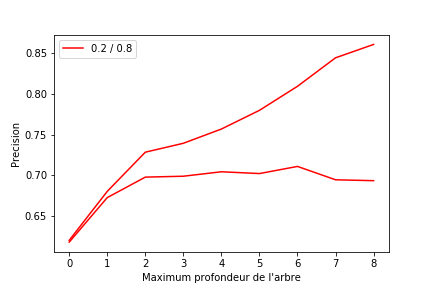
\includegraphics[width=0.8\linewidth]{images/tme1/partition_2_8.png}
	\caption{Donnée aprentissage et test : 0.2 / 0.8}
\end{subfigure}%
\begin{subfigure}{.5\textwidth}
  \centering
	\label{fig:partition_5_5}
	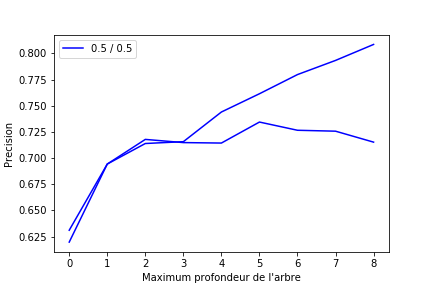
\includegraphics[width=0.8\linewidth]{images/tme1/partition_5_5.png}
	\caption{Donnée aprentissage et test : 0.5 / 0.5}
\end{subfigure}
\begin{subfigure}{.5\textwidth}
  \centering
	\label{fig:partition_8_2}
	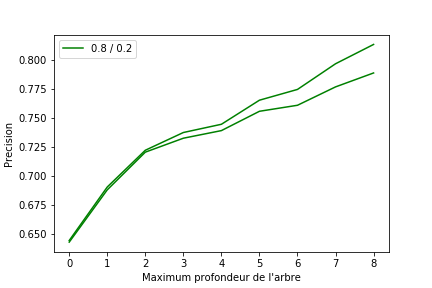
\includegraphics[width=0.8\linewidth]{images/tme1/partition_8_2.png}
	\caption{Donnée aprentissage et test : 0.8 / 0.2}
\end{subfigure}
\begin{subfigure}{.5\textwidth}
  \centering
	\label{fig:partition_vc}
	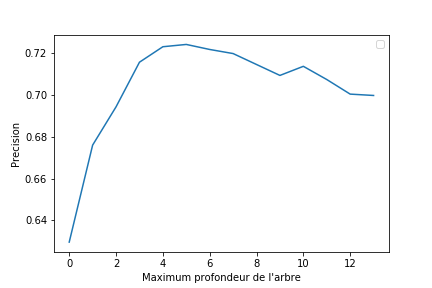
\includegraphics[width=0.8\linewidth]{images/tme1/partition_vc.png}
	\caption{Validation croisee}
\end{subfigure}
\end{figure}

Avec validation croisée on obtient un score plus fiable et stable.
Dans la figure \autoref{fig:tme1_scores} (d) nous pouvons constater, comment le score augmente au début avec la profondeur maximale, mais à la fin il tombe.
Ça c'est à cause de sous et sur apprentissage.
Au début, on généralise beaucoup avec un arbre peu profond (sous apprentissage).
Quand la profondeur se monte sur cinq,
nous commençons à apprendre les données d'apprentissage à la façon trop détaillée et le score sur le test se tombe (sur aprentissage).
La profondeur maximale 4 semble optimal.

\section{TME 2 : Estimation de densité}

Nous sommes intéressés de densité des services différents de Paris.

\subsection{Méthode des histogrammes}

La méthode la plus simple, méthode des histogrammes, il s'agit de partager la valeur continue (latitude et longitude)
à les intervalles fixés et compter, combien d'occurrences chacun contient.

\begin{figure}[h!]
\caption{Densite par méthode des histogrammes}
\label{fig:tme2_histos}
\begin{subfigure}{.5\textwidth}
	\centering
	\label{fig:atms_brut}
	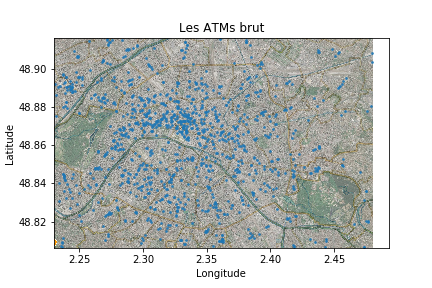
\includegraphics[width=0.8\linewidth]{images/tme2/atms_brut.png}
	\caption{Les ATMs à Paris}
\end{subfigure}%
\begin{subfigure}{.5\textwidth}
  \centering
	\label{fig:atms_histo_5}
	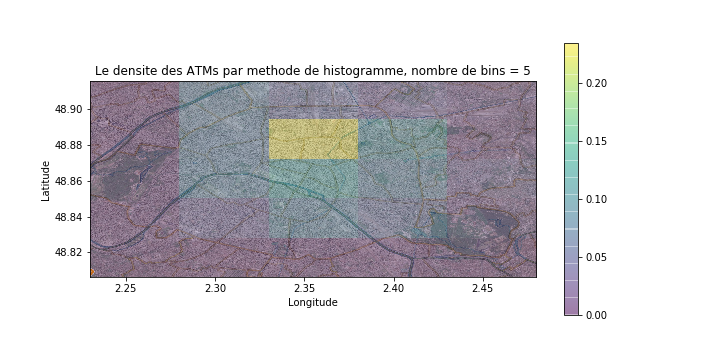
\includegraphics[width=0.8\linewidth]{images/tme2/atms_histo_5.png}
	\caption{Histogramme avec 5 intervalles}
\end{subfigure}
\begin{subfigure}{.5\textwidth}
  \centering
	\label{fig:atms_histo_10}
	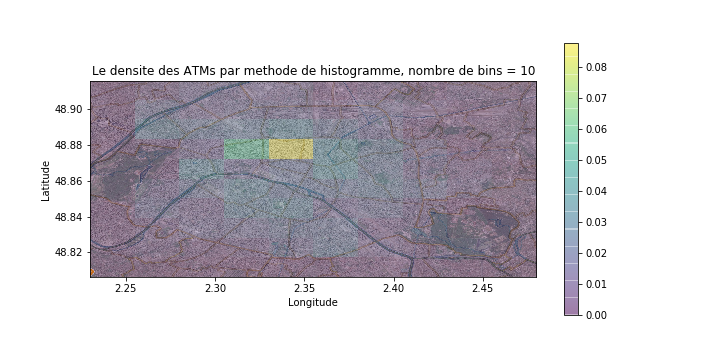
\includegraphics[width=0.8\linewidth]{images/tme2/atms_histo_10.png}
	\caption{Histogramme avec 10 intervalles}
\end{subfigure}
\begin{subfigure}{.5\textwidth}
  \centering
	\label{fig:atms_histo_15}
	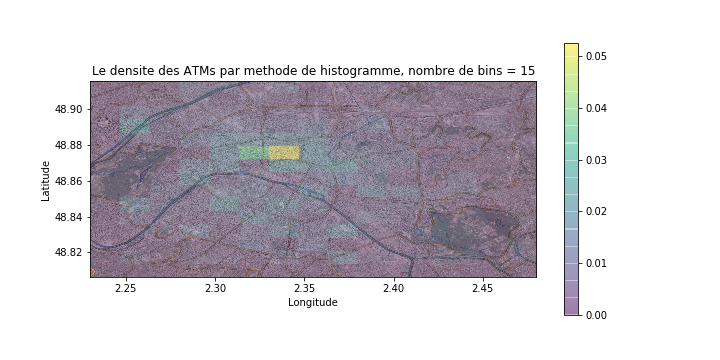
\includegraphics[width=0.8\linewidth]{images/tme2/atms_histo_15.png}
	\caption{Histogramme avec 15 intervalles}
\end{subfigure}
\end{figure}

On peut voir bien avec chaque discretization de \autoref{fig:tme2_histos}, que la densité maximum des ATMs est dans 9iéme arrondissement.
Par contre, la densite n'est pas très visible dans les endroits où la densité est moins forte (par exemple 13iéme arrondissement).
Surtout avec 15 étapes, nous ne voyons pas très bien.

\subsection{Méthode à noyaux}

Comme la méthode de histogramme ne permet pas de visualiser les atms bien avec 15 étapes, je vais fixer le variable étapes à 15 pour l'estimation par noyau.
L'estimation par noyau a une variable h qui est taille de lissage. On va varier d'abord h.

\begin{figure}[h!]
\caption{Parzen comme fonction de Noyau}
\label{fig:tme2_parzen}
\begin{subfigure}{.24\textwidth}
	\centering
	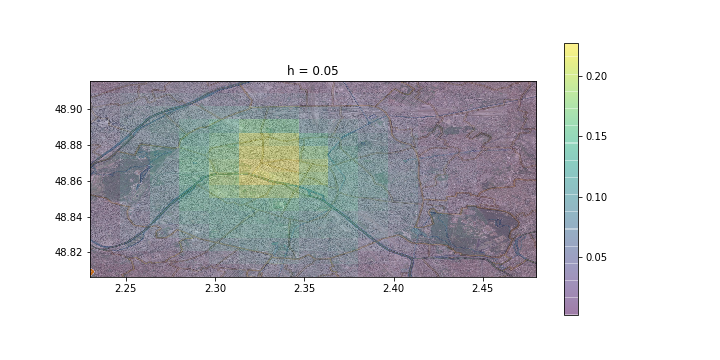
\includegraphics[width=\linewidth]{images/tme2/atms_parzen_0.png}
\end{subfigure}%
\begin{subfigure}{.24\textwidth}
  \centering
	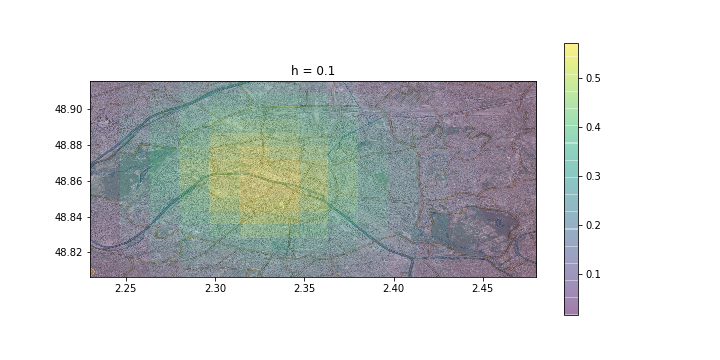
\includegraphics[width=\linewidth]{images/tme2/atms_parzen_1.png}
\end{subfigure}
\begin{subfigure}{.24\textwidth}
  \centering
	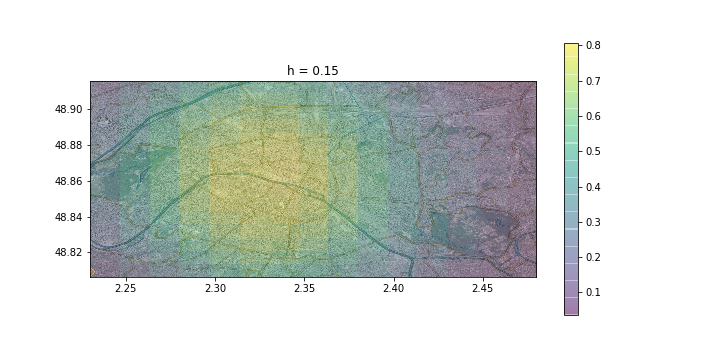
\includegraphics[width=\linewidth]{images/tme2/atms_parzen_2.png}
\end{subfigure}
\begin{subfigure}{.24\textwidth}
  \centering
	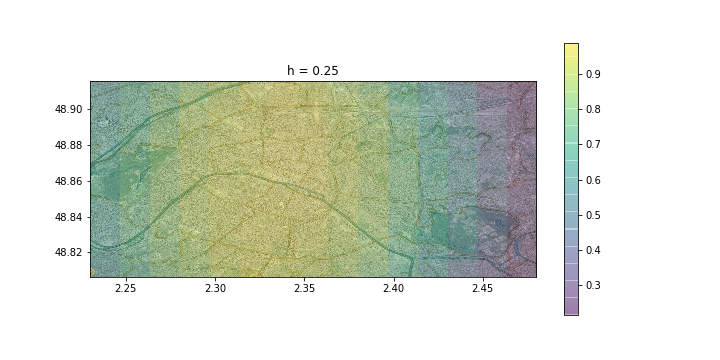
\includegraphics[width=\linewidth]{images/tme2/atms_parzen_3.png}
\end{subfigure}
\end{figure}

Dans \autoref{fig:tme2_parzen}, si h >= 0.25, l'estimation est "oversmoothed".
h = 0.15 l'air le plus optimal, car il prend en compte les points partout à Paris, mais la densité est également visible.

\begin{figure}[h!]
\caption{Gauss comme fonction de Noyau}
\label{fig:tme2_gauss}
\begin{subfigure}{.24\textwidth}
	\centering
	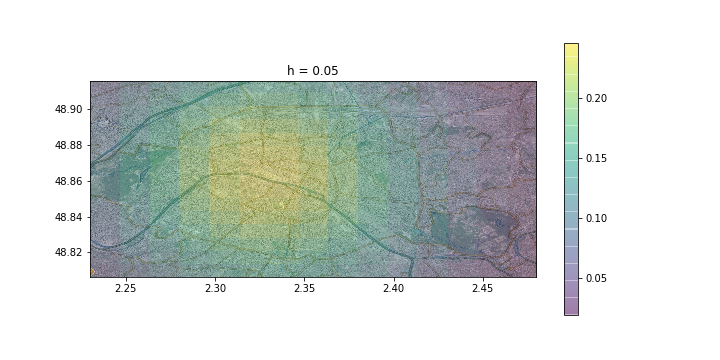
\includegraphics[width=\linewidth]{images/tme2/atms_gauss_0.png}
\end{subfigure}%
\begin{subfigure}{.24\textwidth}
  \centering
	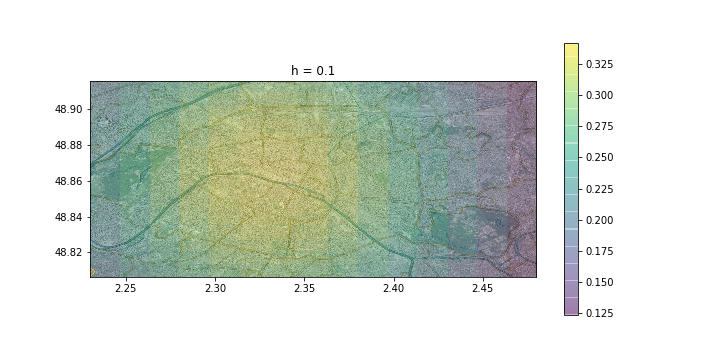
\includegraphics[width=\linewidth]{images/tme2/atms_gauss_1.png}
\end{subfigure}
\begin{subfigure}{.24\textwidth}
  \centering
	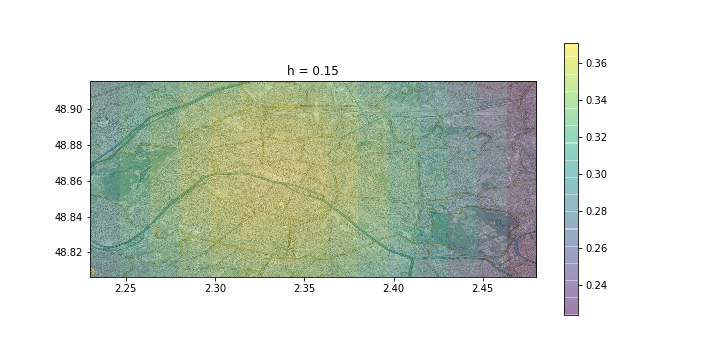
\includegraphics[width=\linewidth]{images/tme2/atms_gauss_2.png}
\end{subfigure}
\begin{subfigure}{.24\textwidth}
  \centering
	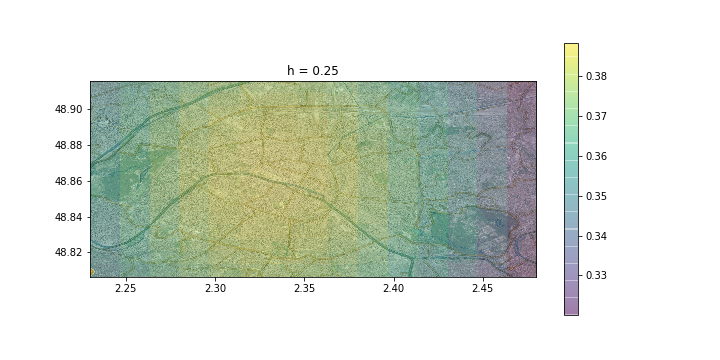
\includegraphics[width=\linewidth]{images/tme2/atms_gauss_3.png}
\end{subfigure}
\end{figure}

Avec le gaussien (\autoref{fig:tme2_gauss}), le meilleur paramètre de lissage est peut-être 0.05.

\subsubsection{Comment choisir de manière automatique le meilleur taille de lissage h ?}

Selon \citep{wiki:kernel_density}, nous pouvons estimer l’optimal taille de lissage h pour noyau de Gauss.
L’estimation est definit dans \autoref{equation:bandwidth_estim}.

\begin{equation}
\label{equation:bandwidth_estim}
h = \left(\frac{4\hat{\sigma}^5}{3n}\right)^{\frac{1}{5}} \approx 1.06 \hat{\sigma} n^{-1/5}
\end{equation}

Nous obtenons h=0.110482310867 pour les données des ATMs à Paris, visualisé dans \autoref{fig:atms_gauss_optimal}.

\begin{figure}[h!]
\caption{Densité avec la méthode de noyaux (Gauss) et lissage optimale}
\label{fig:atms_gauss_optimal}
\centering
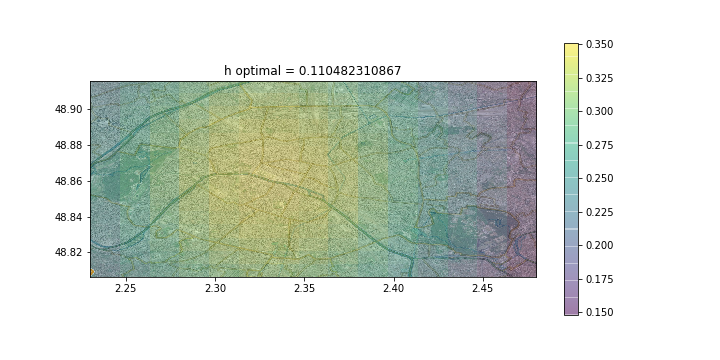
\includegraphics[width=0.6\linewidth]{images/tme2/atms_gauss_optimal.png}
\end{figure}%

L'optimal "rule-of-thumb" estimateur minimise l'erreur de moindre carrée intégré (Mean integrated squared error).
Il permet de montrer le "vraie" distribution, que les POIs vont suivre.
J'ai visualisé également les autres POIs avec le noyaux de Gauss et l'optimal h.
J'ai constaté que les visualisations ne sont pas très différentes.
Les différentes POIs sont distribués à Paris plus ou moins à la même façon :
en centre-ville la densité est grande, d'ailleurs moins.
Donc je pense que ça sera difficile de classifier les POIs seulement par rapport ses localisations.

\section{TME 3 : Descente de gradient}

Cette semaine nous avons implémente la descente de gradient et appliqué ça à régression logistique.

\subsection{Optimisation de fonctions}

Dans le \autoref{fig:tme3_descente} il y a des visualisations de fonctionnement de descente de gradient.
Nous optimisons le fonction f donnée, en cherchent son minimum (locale, car f(x) = x cos(x) n'est pas convexe).
L'axe y correspond la valeur de f(x), donc le minimum local est au fond de courbe et l'axe x correspond les valeurs de x.

\begin{figure}[h!]
\caption{La descente de gradiente de f(x) = x cos(x)}
\label{fig:tme3_descente}
\begin{subfigure}{.33\textwidth}
	\centering
	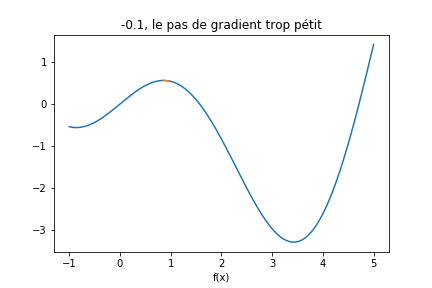
\includegraphics[width=\linewidth]{images/tme3/descente_0.png}
	\caption{}
\end{subfigure}%
\begin{subfigure}{.33\textwidth}
  \centering
	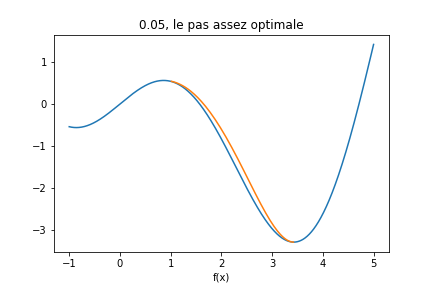
\includegraphics[width=\linewidth]{images/tme3/descente_1.png}
	\caption{}
\end{subfigure}
\begin{subfigure}{.33\textwidth}
  \centering
	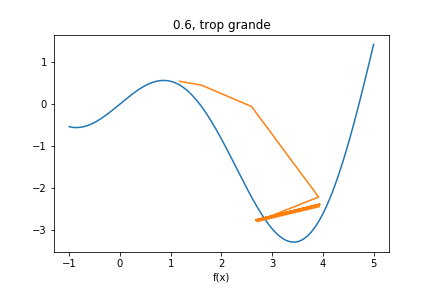
\includegraphics[width=\linewidth]{images/tme3/descente_2.png}
	\caption{}
\end{subfigure}
\end{figure}

Si le bas de descente de gradient est trop petit ou grande,
il y a une risque que, à la fin des itérations d'algorithme, nous n'arrivons pas à minimum de fonction.
(\autoref{fig:tme3_descente} a et c).

Dans le \autoref{fig:tme3_descente_direction} j'ai plotté le direction de descente (defini dans \autoref{equation:descente}) de chaque epsilon de figure
precedent. On peut deduire, que le premier ne descend pas, car son epsilon est negative (direction faux).
Troisiéme descend jusqu'a certain moment, mais apres il commence bugger (epsilon tros grand).
Au milieu, le descente est par contre assez direct vers le minimum.

\begin{equation}
\label{equation:descente}
	\left ( t, \log \left \| x^{t} - x^{*} \right  \| \right )
\end{equation}

\begin{figure}[h!]
\caption{Direction de descente (\autoref{equation:descente})}
\label{fig:tme3_descente_direction}
\begin{subfigure}{.33\textwidth}
	\centering
	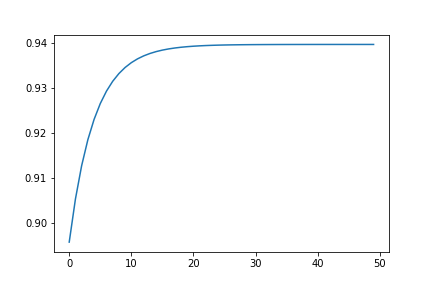
\includegraphics[width=\linewidth]{images/tme3/descente_error_0.png}
\end{subfigure}%
\begin{subfigure}{.33\textwidth}
  \centering
	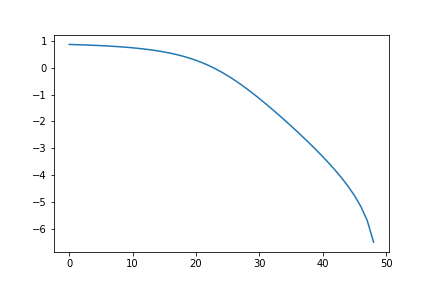
\includegraphics[width=\linewidth]{images/tme3/descente_error_1.png}
\end{subfigure}
\begin{subfigure}{.33\textwidth}
  \centering
	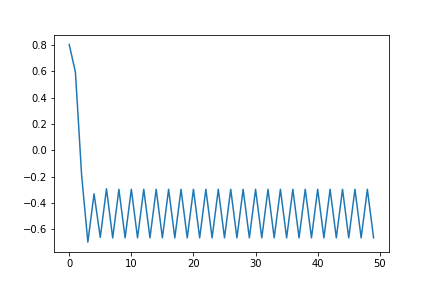
\includegraphics[width=\linewidth]{images/tme3/descente_error_2.png}
\end{subfigure}
\end{figure}

Mon implémentation de descente de gradient ne fonctionne pas parfaitement.
Dans le \autoref{fig:descente_rosenbrock} il y a une optimisation de fonction de Rosenbrock, où on peut voir que l'algorithme ne converge pas à vrai minimum de fonction.
Cette fonction est connue pour ça que c'est difficile de converger à son minimum.

\begin{figure}[h!]
\caption{C'est difficile de converger à minimum de fonction de Rosenbrock}
\label{fig:descente_rosenbrock}
\centering
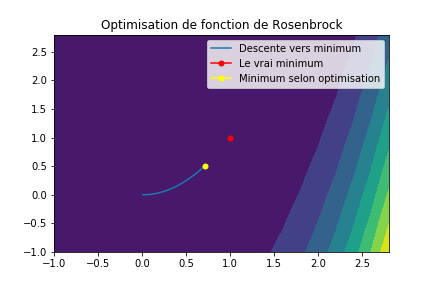
\includegraphics[width=0.4\linewidth]{images/tme3/descente_rosenbrock.png}
\end{figure}%

\subsection{Regression logistique}

J'ai implémente\footnote{Code dans TME3\slash Logistic\_regression.py}
régression logistique, qui utilise la descente de gradient pour optimiser log vraisemblance.

Je vais comparer classification des nombres différents (les données USPS).
Pour le pas de descente de gradient j'ai fixé eps = 0.025 qui fonctionne bien avec différents nombres.

Pour chaque combination $$\left ( i,j \right ) \in \left \{ 0...9 \right \} \times  \left \{ 0...9 \right \}$$
nous calculons dans \autoref{fig:logistique_numbers} les scores avec cinq iteration de validation croisée.

\begin{figure}[h!]
\caption{Les nombres un contre un}
\label{fig:logistique_numbers}
\begin{subfigure}{.5\textwidth}
	\centering
	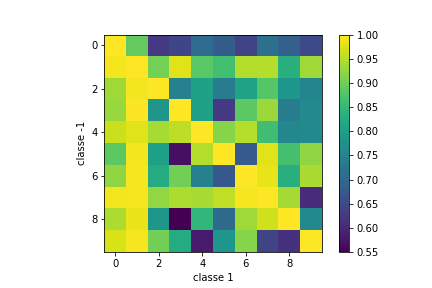
\includegraphics[width=\linewidth]{images/tme3/logistic_one_vs_one.png}
	\caption{Regression logistique}
\end{subfigure}%
\begin{subfigure}{.5\textwidth}
  \centering
	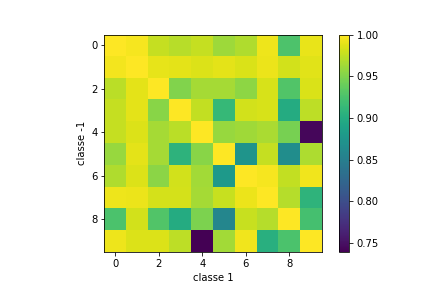
\includegraphics[width=\linewidth]{images/tme3/nb_one_vs_one.png}
	\caption{Naif Bayes}
\end{subfigure}
\end{figure}

Nous pouvons constater dans \autoref{fig:logistique_numbers} a), avec regression logistique, par exemple que le nombre 5 étant classe -1 et 3 étant classe 1 on obtiens score mal.
Également le nombre zéro est difficile de classifier, comme on peut voir dans \autoref{fig:logistique_numbers} a) sur
le premier ligne. La difficulté avec zéro est probablement à cause de fait, qu'on a beaucoup plus de zeros dans les données que les autres et la forme de zero est distribué largement
et est donc facile de mélanger avec les autres.
Naif bayes semble fonctionner mieux sur classification un contre un (\autoref{fig:logistique_numbers} a)).
Seulement le score entre 4 et 9 est moins elevée.

\begin{figure}[h!]
\caption{Les nombres, un contre les autres}
\label{fig:USPS_one_vs_all}
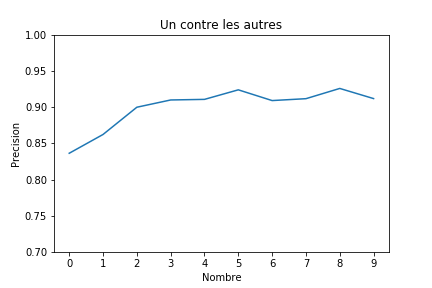
\includegraphics[width=0.5\linewidth]{images/tme3/USPS_one_vs_all.png}
\centering
\end{figure}%

Dans \autoref{fig:USPS_one_vs_all} il y a comparison entre les scores de regression logistique et naif bayes
\footnote{Code dans TME3\slash NaiveBayes\_classifier.py}. Nous calculons le precision (avec validation croisée de cinq scores)
de chaque nombre comparée à tous les autres nombres. Ça va dire, que nous mettons le classe -1 pour cet nombre et classe 1 pour tous les autres.
En moyenne, le regression logistique est plus stable et robust, mais parfois on obtient meilleur resultat avec classificateur
de naif bayes (comme pour nombre 1 : avec NB c'est presque parfait le classification).

\section{TME 4 et 5 : Perceptron}

\section{TME 5 : Support Vector Machine}


\subsection{Pistes de recherche}

\bibliographystyle{plainnat}
\bibliography{biblio}

\end{document}
